%% LyX 2.0.2 created this file.  For more info, see http://www.lyx.org/.
%% Do not edit unless you really know what you are doing.
\documentclass[12pt,twoside,english]{report}
\usepackage{lmodern}
\renewcommand{\familydefault}{\rmdefault}
\usepackage[T1]{fontenc}
\usepackage[latin9]{inputenc}
\usepackage[a4paper]{geometry}
\geometry{verbose,tmargin=3.5cm,bmargin=3cm,lmargin=3.5cm,rmargin=3cm,footskip=1cm}
\usepackage{fancyhdr}
\pagestyle{fancy}
\setcounter{secnumdepth}{3}
\setcounter{tocdepth}{3}
\setlength{\parskip}{\medskipamount}
\setlength{\parindent}{0pt}
\usepackage{float}
\usepackage{tipa}
\usepackage{textcomp}
\usepackage{amsmath}
\usepackage{graphicx}
\usepackage{setspace}
\usepackage[authoryear]{natbib}
\usepackage{nomencl}
% the following is useful when we have the old nomencl.sty package
\providecommand{\printnomenclature}{\printglossary}
\providecommand{\makenomenclature}{\makeglossary}
\makenomenclature
\setstretch{1.5}

\makeatletter
%%%%%%%%%%%%%%%%%%%%%%%%%%%%%% User specified LaTeX commands.
\usepackage{fancyhdr}
\pagestyle{fancy}
\fancyhead[RE]{\bfseries \nouppercase\leftmark}
\fancyhead[LO]{\bfseries \nouppercase \rightmark}

\renewcommand{\chaptermark}[1]{%
\markboth{\chaptername 
\ \thechapter\ }{}}

 
\fancyhead[LE,RO]{\bfseries\thepage}
\fancyfoot{}
\raggedbottom
\setlength{\parindent}{8mm}

\makeatother

\usepackage{babel}
\begin{document}

\chapter{Self-Organising Maps and Classifying the Synoptic Weather Systems
of Australia\label{chap:SOM-Synoptic-Weather-Aus}}

\newpage{}


\section*{Summary}

\noindent This chapter examines the Self-Organising Map (SOM) technique
and how it is utilised in climatology in general, and how it has been
applied in the context of Australia. The SOM algorithm is described
in full and previous research comparing the performance of the SOM
to other commonly used techniques is presented. This chapter also
introduces the reanalysis data used for Part 1 and the performance
of the data in comparison to other data sets. \newpage{}


\section{History of the SOM\label{sec:History-of-the-SOM}}

First proposed by Teuvo Kohonen in the late 1980\textquoteright{}s
the SOM acts in a similar manner to most data reduction techniques
in its attempt to synthesise a large multidimensional data-set into
a series of discrete, commonly occurring, modes of variability. With
its origins in the study of brain activity, the SOM can also be called
an artificial neural network due to its 2D grouping of cells that
are specifically tuned by various input signals (\citealp{Kohonen1990}).
By successively ``showing'' the data to the SOM array and then altering
the 2D array to look more like the data, the SOM technique aims to
identify specific patterns from within the data that are the most
common. 

The seminal use of SOMs in synoptic climatology was by \citet{Hewitson2002}.
\citet{Hewitson2002} used the SOM technique to categorise a gridded
Mean Sea-Level Pressure (MSLP) data-set of the northeast United States
into 35 archetypal pressure distributions. \citet{Hewitson2002} found
the SOM to be a very useful method for determining common synoptic
regimes as it presented an array of pressure maps that span the data-space
and thus a continuum of synoptic maps was produced rather than, say,
a group of clusters that have less obvious relationships to one another.
Since \citet{Hewitson2002} the SOM technique has become increasingly
popular in climatology; a field in which it is more popular to find
Principle Component based clustering techniques (\citealp{Sheridan2011}).
Specifically, the SOM has been widely used for the study of pressure
patterns that co-occur with precipitation events (\citealp{Sheridan2011}). 


\section{SOM Methodology\label{sec:SOM-Methodology}}

The training of the SOM in the current study occurred in two main
phases, in accordance with the suggestions from the software and the
works of \citet{Hewitson2002} and \citet{Alexander2010}. The first
phase involved a random initialisation of each SOM node, followed
by training with the data. The training in the SOM algorithm is conducted
by sequentially presenting the time-steps from the data to be mapped
(in this case the ERA-Interim MSLP data), followed by a search for
the SOM node that best matches each data sample. The node that best
matches (hereafter referred to as the Best Matching Unit \nomenclature{BMU}{Best Matching Unit}(BMU))
is determined by the Euclidean distance measurement; shown here in
Eq. 1 from \citet{Kohonen1995}: 
\begin{eqnarray}
\text{\textdoublepipe}x-m_{c}\text{\textdoublepipe} & = & \underset{i}{min}\left\{ \text{\textdoublepipe}x-m_{i}\text{\textdoublepipe}\right\} \text{{,\,\,\,\ or}}\nonumber \\
c & = & arg\,\underset{i}{min}\left\{ \text{\textdoublepipe}x-m_{i}\text{\textdoublepipe}\right\} \label{eq:1-BMU}
\end{eqnarray}


where $c$ is the argument of the winning node, $x$ is the data sample
and $m_{i}$ is the node that $x$ is being compared with; indicating
that $m_{c}$ would be the BMU.

The BMU and the nodes that surround the BMU are then altered to look
more like the data. The amount the nodes are altered by is determined
by two parameters: namely, the alpha value and radius value. The alpha
value decreases linearly from an initial value to zero during training
and the radius value is given the value of the smallest dimension
size of the SOM in training phase one. In this thesis the choice was
made to utilise a Gaussian approach to node alteration (Eq. \ref{eq:3-Gaussian-Function}).
In the Gaussian approach the alpha and radius values control the decay
rate of the Gaussian function, centred on the BMU, such that nodes
immediately surrounding the BMU are altered much more than those further
away in the SOM space. An alternative approach to the Gaussian utilises
just a monotonically decreasing function of $t$ ($h_{ci}(t)=\alpha(t)$
only) and is termed the 'Bubble' approach. In this thesis the Gaussian
approach was selected because it was found to produce SOMs with consistently
smaller Euclidean distances to the original data (not shown). The
amount that each node is altered can be described by Eqs. 2 and 3
from \citet{Kohonen1995}:

\begin{equation}
\begin{array}{cccc}
m_{i}(t+1)=m_{i}(t) & + & h_{c}(t)\,[\, x(t)-m_{i}(t)] & ,\,\, and\,\,\end{array}\label{eq:2-Node-Alteration}
\end{equation}


\begin{equation}
\begin{array}{ccccc}
h_{ci}(t)=\alpha(t) & \cdot & \exp(-\frac{\parallel r_{c}-r_{i}\parallel^{2}}{2\sigma^{2}(t)})\end{array}\label{eq:3-Gaussian-Function}
\end{equation}


\noindent \,\,\,\,\,\,\,\,where $c$, $i$, $x$, and $m$
are as before, $t$ is an integer value between $0$ and the run length,
$\alpha(t)$ and $\sigma(t)$ are monotonically decreasing functions
of $t$ $(0<\alpha(t)<initial\,\, alpha)$ and $N_{c}$ are the neighbourhood
array points around node $c$ that are contained within the initial
radius, $r$. The run length describes how many times the data are
shown to the SOM and in the first phase was equal to the number of
time steps in the ERA-Interim data (i.e. each time step was shown
once and hence $t$ from Eqs. \ref{eq:2-Node-Alteration} and \ref{eq:3-Gaussian-Function}
can represent the time-steps in the data). Each successive pass of
the data alters the BMU and surrounding nodes, according to the above
equations, such that the SOM nodes start to resemble the data. Various
initial alpha values were tested in the current study---in accordance
with \citet{Alexander2010}: 
\[
initial\,\, alpha=(0.001,0.002,...,0.01,0.02,...,0.1,0.15,0.2,...,1)
\]
\,\,\,\,\,\,\,\,The second training phase is conducted in
a similar manner to that of the first phase, with the exception that
the starting point of the SOM is the state of the SOM at the end of
the first training phase. In the second phase the run length is also
increased to be 10 times the number of time steps in the data, the
radius value is reduced to one and the alpha value is half that of
the initial alpha value. The second training phase could therefore
be thought of as a process for adding in the finer detail that is
missed from the initial training phase. 

The outcome of the SOM procedure is a matrix of related MSLP distributions.
The size of the matrix (number of nodes in the SOM space) is predetermined
by the user and once established the SOM nodes can be mapped back
onto the original data (assigning a SOM node to each time step via
the BMU method). The mapping of the SOM nodes back onto the original
data converts the data into a time series of SOM nodes (weather types),
allowing for the time-wise behaviour of common weather types to be
examined. In the case of this thesis, the SOM method enables the identification
of common characteristics in an otherwise complicated MSLP dataset,
which in turn also enables a study of related variables (wind and
solar) and how they vary in association with the common weather types.


\section{The SOM in Australia\label{sec:SOM-in-Aus}}

In terms of the Australian region, there have been a small number
of noteworthy studies that have utilised the SOM technique. For instance,
\citet{Alexander2010} used the ECMWF product ERA-40 to produce a
20 member SOM of MSLP (Fig. \ref{fig:Alexander-SOM}). Comparably
the works of \citet{Brown2010} (Fig. \ref{fig:Brown-SOM}) and \citet{Nicholls2009}
(Fig. \ref{fig:Nicholls-SOM}) produced SOMs with very similar features.
As opposed to the \citet{Alexander2010} and \citet{Nicholls2009}
studies the \citet{Brown2010} study used National Centre for Environmental
Prediction MSLP data for the Australian region. Importantly though
the SOM from the \citet{Brown2010} paper contains many of the same
features to the ERA-40 derived SOMs in \citet{Alexander2010} and
\citet{Nicholls2009}. Other notable studies using the SOM technique
in the Australian region include \citet{Hope2006}, which utilised
a 20 member SOM of Western Australian MSLP and \citet{Verdon-Kidd2009},
which implemented a 20 member SOM of Victorian MSLP. 
\begin{figure}[H]
\begin{centering}
\includegraphics{\string"Figures/Alexander SOM\string".eps}
\par\end{centering}

\caption{SOM nodes for the winter months of 1958-2001 using Mean Sea-Level
Pressure data (hPa) from ERA-40. Numbers in brackets represent percentage
occurrence for 1907-2006 and ``m'' represents the decadal trend
in that node. Figure originally presented in \citet{Alexander2010}.
\label{fig:Alexander-SOM}}
\end{figure}
\begin{figure}[h]
\noindent \centering{}\includegraphics{\string"Figures/Brown SOM\string".eps}\caption{20 member SOM of 1979-2008 National Centre for Environmental Prediction
reanalysis MSLP. F values represent the frequency occurrence of the
SOM node. Figure originally presented in the \citet{Brown2010} study.\label{fig:Brown-SOM}}
\end{figure}
\begin{figure}[h]
\noindent \centering{}\includegraphics{\string"Figures/Nicholls SOM\string".eps}\caption{20 member SOM of 1979-2001 ERA-40 MSLP. Figure originally presented
in the \citet{Nicholls2009} study.\label{fig:Nicholls-SOM}}
\end{figure}


With the results from previous studies in mind it was decided that
the SOM would also be a suitable technique for the current study.
The SOM's ability to summarise large data sets into a limited number
of commonly occurring weather types (via the MSLP field) was identified
as being useful for analysing the common wind and solar distributions,
as well. In a similar manner to the studies of \citet{Alexander2010},
\citet{Hope2006}, and \citet{Verdon-Kidd2009} later chapters identify
common MSLP patterns. However, instead of analysing the co-occurrence
of precipitation, the wind speed and solar irradiance fields are analysed
for how they relate to the common weather regimes.


\section{The SOM Compared to Other Techniques}

Synthesis of a large data set into a limited number of commonly occurring
features of that data set is a process frequently utilised in science,
and in particular climatology. While the SOM technique has only recently
been applied to the field of climatology there are other techniques,
for the purposes of data synthesis, that have been in use for much
longer. One such technique is Principle Component Analysis \nomenclature{PCA}{Principle Component Analysis}(PCA).
A study comparing the PCA technique to the SOM was recently conducted
for eastern Australia by \citet{Jiang2012}. \citet{Jiang2012} used
PCA analysis to estimate the number of weather types needed for eastern
Australia (12) and then use k-means clustering to form 12 clusters/synoptic
types of the 1958-2009 NCEP/NCAR reanalysis 100hPa geopotential height.
For the SOM \citet{Jiang2012} use the standard procedure of two-phase
training, like that outlined above. \citet{Jiang2012} then utilised
a 12-node SOM for comparison with the 12 clusters from the PCA analysis
(\citet{Jiang2012} also tests a 20-node SOM). \citet{Jiang2012}
found that in general the SOM technique had more advantages than the
PCA-clustering approach. In particular it was highlighted that the
SOM can be used as a clustering tool if the radius ($r$) is set to
zero, and when utilised in this way the SOM had similar performance
to the k-means clustering approach. Where the SOM differed was in
its ability to produce transition patterns---geopotential height patterns
that fall between the dominant features. By spanning the data space
the SOM is more useful for studies that want to analyse weather pattern
trajectories, as well as studies that wish to understand the influence
of more subtle features (\citet{Jiang2012}).

In a similar study, but for the European region, \citet{Rousi2013}
also found the SOM to be more advantageous than the PCA approach.
\citet{Rousi2013} found that the both the SOM and the PCA were able
to identify the main mode of variability for the region (the North
Atlantic Oscillation), but that the SOM was able to also identify
smaller features that the PCA missed because of its more discrete
representation---a similar finding to \citet{Jiang2012}. Other techniques
also exist for the purposes of data synthesis, including simulated
annealing clustering. \citet{Philipp2007} presented a comprehensive
study of simulated annealing clustering in comparison to k-means clustering
for the north Atlantic. \citet{Philipp2007} found the simulated annealing
clustering to be a far more robust technique, however, a direct comparison
of this technique with the SOM appears not to exist yet. 

It has been shown that for the purposes of this thesis the SOM technique
will be an appropriate tool for classifying the major, as well as
the transitional, modes of variability for the Australian region.
By capturing both the major modes of variability, as well as transitions
therein, the SOM will provide a comprehensive assessment of synoptic
scale variance over Australia. The SOM will therefore also enable
a comprehensive assessment of the synoptic scale influences on wind
speed and solar irradiance.


\section{Data for Part 1\label{sec:Data-for-Part1}}

The data used in the current study are from the European Centre for
Medium-range Weather Forecasts (ECMWF). Specifically, the ERA-Interim
product was chosen to conduct the climatology of the Australian region.
ERA-Interim is a global reanalysis product that spans the period 1989
to almost current day and which is freely available to non-ECMWF members
at 1.5� Latitude/Longitude (\textasciitilde{}166km) spatial resolution
(\citealp{Berrisford2009}); although recently the ERA-Interim archive
has been extended back to 1979. 

As noted in \citet{Simmons2006} reanalysis products are superior
to other global products, such as high-resolution operational forecasting
systems, for studies into the long-term climate because reanalyses
do not involve the continual adjustment to higher resolution systems
that follow improvements in computing power. Rather, reanalysis products
offer a stable platform upon which a single version of the data assimilation
system is used (\citealp{Dee2011}). It is for this reason that reanalysis
products are able to provide a long-term and coherent record of the
global atmospheric circulation (\citealp{Dee2011}). Having said that,
reanalysis products are far from fault-free. Indeed the analysis systems
suffer from model biases, limits to and changes in the coverage of
observations and thus for some variables the analysis of long-term
trends can produce spurious results (\citet{Trenberth2011}).

The ERA-Interim reanalysis used in the current study is the third
global reanalysis that has been produced by ECMWF. As noted in \citet{Dee2011}
ERA-Interim improves upon the previous reanalysis product, ERA-40,
in many aspects. For instance, in ERA-Interim the atmospheric model
is coupled to an ocean-wave model, which was not the case in ERA-40
(\citealp{Berrisford2009}). ERA-Interim also includes the introduction
of 4-dimensional variational analysis (4D-Var) and a variational bias
correction scheme for satellite-derived radiances---both of which
were not included in ERA-40. As a consequence, \citet{Dee2011} were
able to show improved temporal consistency on synoptic time-scales.
\citet{Dee2011} were also able to show that the background departures,
defined as being the difference between the forecast of the next observation
and the observation, are smaller in ERA-Interim. 

In terms of the performance of ECMWF products in comparison to observations
it was found by \citet{Kiss2009} that low-level wind speeds from
ERA-40 reanalysis and were able to reproduce the appropriate dynamics
seen in observations from two wind turbines in Hungary. Unfortunately,
published comparisons between the ERA-Interim near-surface wind speeds
and observations are, and in particular for the Australian region,
limited in number. \citet{Dee2011} noted that the background departures
for globally averaged ERA-Interim surface winds are smaller than ERA-40.
\citet{Dee2011} also reported some decreasing trends in surface winds
for ERA-Interim for the period 1992-2002 when compared to the European
Remote Sensing satellite and QuickScat data---although the trends
then reversed after 2002, noted as likely due to the evolution in
the observing system. Some analysis presented below shows that the
relatively coarse resolution of the ERA-Interim model (\textasciitilde{}80km
spatially) compares well with the former regional model of the Bureau
of Meteorology (MesoLAPS\_125, 12.5km spatially) for the same dates
(Fig, \ref{fig:U10-comp-ERA-Meso}). While Fig. \ref{fig:U10-comp-ERA-Meso}
is not a comparison with observations it does test model resolution
dependence---showing that for large scale features the ERA-Interim
resolution captures that which a finer model resolution can capture.
\begin{figure}[h]
\noindent \begin{centering}
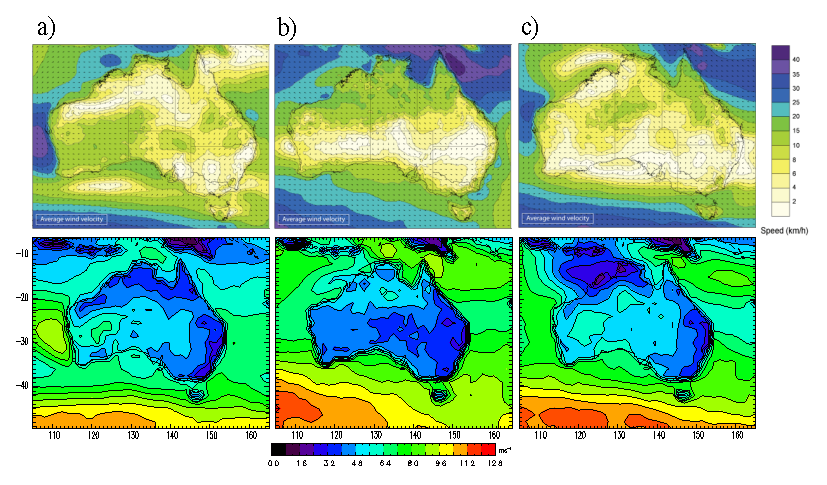
\includegraphics{Figures/U10_average_comp_era_meso}
\par\end{centering}

\caption{Comparison of average 10m wind speed for MesoLAPS\_125 (top panel)
and ERA-Interim (bottom panel), for the months of a) January, b) July
and c) October during 2004-2008.\label{fig:U10-comp-ERA-Meso}}
\end{figure}
 

In terms of the surface solar radiation fields from ERA-Interim \citet{Dee2011}
examined the energy balance at the surface. \citet{Dee2011} showed
that while there was a larger positive bias in the net solar radiation
at the surface for ERA-Interim when compared to ERA-40, these biases
were most prevalent over the ocean. Over land areas---the primary
concern of this thesis is the Australian continent---the surface energy
balance has improved in ERA-Interim (0.5 Wm\textsuperscript{-2},
from 1.3Wm\textsuperscript{-2} in ERA-40). Indeed, while the surface
energy balance over the ocean might be poor in ERA-Interim when compared
to ERA-40, \citet{Balmaseda2010} were able to show that the ERA-Interim
spatial structures and the representation of seasonal and interannual
variability in surface fluxes (over the ocean) have improved from
ERA-40. Despite analysis systems not being designed to conserve quantities
like energy, mass and angular momentum, in general the ERA-Interim
budget closure is better than ERA-40 (\citealp{Dee2011}).

While there are noted model biases and inevitable flaws in the process
of running a global model with inconsistent observational coverage,
it should be stressed that such challenges are present for all reanalysis
systems, not just ERA-Interim. In previous paragraphs the ERA-interim
reanalysis archive has been shown to perform well in a number of relevant
variables for this thesis. As such, for the purposes of Part 1---synoptic
typing of MSLP and the large-scale interpretation of coincident DSR
and near-surface wind speed for Australia---the ERA-Interim reanalysis
will be used.
\end{document}
